\begin{titlepage}
    \thispagestyle{empty}
    
    \vfill
    \begin{center}
        \rule{\textwidth}{1.6pt}\vspace*{-\baselineskip}\vspace*{2pt}
        \rule{\textwidth}{0.4pt}\par\vspace{\baselineskip}
        {\Huge \scshape Volume I: Memory Fields}\par\vspace{0.2in}
        {\Large \itshape Differentiable Latent Indexing inside Large Language Models}\par\vspace{3.2pt}
        \rule{\textwidth}{0.4pt}\vspace*{-\baselineskip}\vspace{3.2pt}
        \rule{\textwidth}{1.6pt}
    \end{center}
    \vfill
\end{titlepage}

\chapter*{Abstract}
This article proposes \textit{Differentiable Latent Indexing} (DLI), a theoretical framework that recontextualizes memory retrieval not as an external utility appended to a language model, but as a native, differentiable function inside the computational pathway of Large Language Models (LLMs). By treating latent space as a structured information field, the article derives formal retrieval operators through which memory access can be integrated directly into the model's forward pass.

The central claim is that the conventional separation between storage and processing introduces architectural inefficiencies that limit the development of autonomous and cognitively organized AI systems. In current retrieval-augmented designs, the model, retriever, embedding store, and generator often remain operationally coupled but mathematically discontinuous. DLI instead proposes a shared latent memory substrate in which retrieval, routing, and representation learning are jointly optimized.

This work is presented as a conceptual research article. It does not claim empirical validation. Instead, it establishes mathematical scaffolding, explicit propositions, falsification conditions, implementation pathways, and expected failure modes for future experimental work. In doing so, it serves as the first component of a broader research program investigating the internal organization of machine cognition.

\noindent \textit{Keywords: Differentiable Latent Indexing (DLI); Large Language Models (LLMs); Retrieval-Augmented Generation (RAG); Cognitive Architectures; Neural Retrieval; Differentiable Memory; Transformer Models; Cognitive Complete AI; Hypothesis-Extension Research; Artificial Intelligence Theory.}

\vspace{2em}
\hrule
\vspace{2em}

\chapter{Propositions}

\section*{Proposition 1: Retrieval Efficiency Gain}
If DLI provides a meaningful internal memory mechanism, models augmented with DLI should demonstrate improved performance on tasks requiring long-range dependency resolution compared with baseline transformers of equivalent parameter count.

\textbf{Falsification condition:} If no statistically significant improvement is observed across controlled benchmarks, the hypothesis that internally differentiable retrieval improves effective memory capacity is weakened.

\section*{Proposition 2: Latent Clustering Stability}
DLI should induce measurable clustering in latent representations corresponding to recurrent semantic structures.

\textbf{Falsification condition:} If latent representations remain uniformly distributed or indistinguishable from baseline attention patterns, the claim of structured internal memory is not supported. To mathematically verify this organization, the spatial distribution of the latent memory field can be monitored via a localized Silhouette Coefficient ($S$). For a cluster of recurrent semantic structures $C$, the stability metric is formalized as:

\begin{equation}
S(M^{(\ell)}) = \frac{1}{|C|} \sum_{i \in C} \frac{b(i) - a(i)}{\max(a(i), b(i))},
\end{equation}

where $a(i)$ represents the mean intra-cluster distance of representation $i$, and $b(i)$ represents the mean nearest-cluster distance to any other semantic partition. The proposition holds if and only if $S(M^{(\ell)}) > \epsilon$ as training progress approaches convergence, where $\epsilon$ is the baseline uniform distribution threshold.

\section*{Proposition 3: Retrieval-Induced Drift}
Repeated retrieval operations should introduce measurable drift in latent state trajectories.

\textbf{Falsification condition:} If no measurable deviation from baseline forward-pass dynamics is observed, the proposed retrieval interaction is not functionally distinct.

\section*{Introduction}
The present work inaugurates a trilogy of conceptual research articles that together outline a research trajectory centered on latent cognition in artificial systems. This first article formalizes \textit{Differentiable Latent Indexing} (DLI) as a native retrieval mechanism inside Transformer-based language models. The article does not report experimental results; rather, it formalizes, elaborates, and critically develops a hypothesis into a coherent architectural framework. In this sense, the work belongs to a theoretical tradition in which formal models precede experimental construction.

The paper extends the Differentiable Latent Indexing inside Large Language Models (DLI-LLM) hypothesis by positioning it as an architectural paradigm for retrieval inside Transformer computation. The second article in this series will examine \textit{Curriculum-Induced Symbol Invention} (CISI) as a mechanism for emergent reasoning primitives. The third article will synthesize both threads into a broader account of how memory and symbols may be integrated in artificial cognition. Together, these papers aim to establish a conceptual lineage for AI systems that treats memory, routing, representation, and control as interdependent components of machine cognition.

This article was developed in response to a hypothesis generated by the Academia.edu AI-assisted scientific modeling platform. The originating hypothesis proposed a learnable, differentiable memory retrieval mechanism embedded directly within Transformer layers. Rather than treating that hypothesis as a fixed endpoint, the present paper treats it as a conceptual seed: a starting point from which to examine the architectural, cognitive, mathematical, and safety implications of internalized retrieval.

The problem space addressed here is the separation between parametric memory, stored within model weights, and non-parametric memory, retrieved through external documents, embedding stores, or vector databases. Retrieval-augmented generation has improved factual grounding by combining sequence-to-sequence generation with external dense retrieval \cite{Lewis2021}. Related approaches, including nearest-neighbor language models and memorizing transformers, demonstrate that language models can benefit from access to stored representations beyond the immediate context window \cite{Khandelwal2020,Wu2022}. However, these approaches also preserve a structural separation between the model's internal computation and the retrieval substrate.

This separation produces three persistent architectural constraints:

\begin{enumerate}
    \item latency and bandwidth trade-offs between inference and retrieval operations;
    \item semantic drift between retrieved information and the evolving internal context of the model; and
    \item limited gradient flow between evidence selection, memory access, and downstream reasoning.
\end{enumerate}

DLI proposes a departure from this pattern. It introduces a differentiable memory module embedded within Transformer layers and trained jointly with the model. Memory queries are formulated from hidden states, routed toward a latent key--value memory, and fused back into the model through gated integration. Product quantization provides a possible mechanism for scalable approximate search, while gating regulates when retrieved memory should influence the hidden state \cite{Jgou2011,Johnson2021,Lepikhin2020}.

By situating retrieval as an internalized cognitive function, DLI reframes memory access as part of the model's own computational graph rather than as an external service call. The resulting architecture is not merely an optimization of retrieval-augmented generation. It is a theoretical proposal for unifying attention, memory, and representational control inside Transformer-based systems.

\section*{Contributions}
This work contributes the following elements:

\begin{enumerate}
    \item a unified architectural hypothesis that integrates latent memory directly into Transformer computation;
    \item a mathematical definition of differentiable retrieval, routing, and gated fusion;
    \item a conceptual implementation blueprint for internal retrieval during inference;
    \item a comparative analysis connecting DLI to retrieval-augmented generation, kNN language models, differentiable memory systems, recurrent memory transformers, and cognitive architectures; and
    \item a foundation for the broader research program developed in the \textit{Latent Cognition Trilogy}.
\end{enumerate}

\section{Overview of the Paper}
Section 2 develops the methodological foundation by decomposing the originating DLI-LLM hypothesis into its constituent architectural claims. Section 3 presents theoretical predictions and falsifiable implications. Section 4 develops the mathematical formulation of Differentiable Latent Indexing. Section 5 provides a conceptual implementation blueprint and comparative literature analysis. Section 6 discusses broader implications for cognitive modeling, learning dynamics, safety, and cognitive-complete Transformer architectures.

\section{Theoretical Construction and Implications}
This paper does not report empirical results. Its contribution is the theoretical development of a Transformer-based architecture through structured hypothesis modeling. The starting point is the DLI-LLM hypothesis, which is decomposed into a set of architectural claims and then expanded into a formal framework suitable for future empirical study.

\subsection{Hypothesis Decomposition}
The original hypothesis can be decomposed into four architectural claims:

\begin{enumerate}
    \item a differentiable memory module embedded inside Transformer layers;
    \item a product-quantized memory structure for scalable approximate retrieval;
    \item a shared latent vector space for token-level representations and document-level embeddings; and
    \item a learned query-gating mechanism for retrieval triggering and fusion control.
\end{enumerate}

Each claim has precedent in adjacent literature but differs in the proposed integration. Neural Turing Machines and Differentiable Neural Computers introduced differentiable access to external memory \cite{Graves2014,Graves2016}. Memory-augmented neural networks demonstrated rapid assimilation of new examples through content-based memory access \cite{Santoro2016}. Recurrent memory transformers and memorizing transformers later adapted memory mechanisms to Transformer-based language modeling \cite{Bulatov2022,Wu2022}. DLI differs from these systems by treating latent retrieval as an internal and trainable component of the Transformer layer itself.

\subsection{Architectural Modeling}
The hypothesis is extended into a multi-stage retrieval loop inside the forward pass. At a high level, the current hidden state generates a query vector. That query vector retrieves top-$k$ value vectors from a latent key--value memory. The retrieved representation is then fused back into the model through a learned routing gate. This loop creates a differentiable pathway between hidden-state evolution and memory access.

The proposed retrieval loop contains three major operations:

\begin{enumerate}
    \item cross-layer memory interpolation, in which retrieval results influence subsequent Transformer layers;
    \item sparse top-$k$ selection, allowing retrieval to remain computationally bounded; and
    \item internal--external evidence arbitration, in which latent memory competes with or complements the local attention pathway.
\end{enumerate}

To visualize the core concept, \textbf{Figure}~\ref{fig:dli-architecture} introduces the proposed DLI-LLM architecture.

\begin{figure}
    \centering
    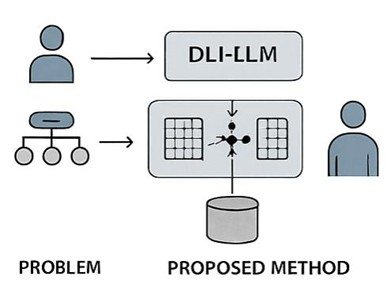
\includegraphics[width=0.72\linewidth]{volumes/pic/Picture1.1.jpg}
    \caption{Differentiable Latent Indexing architecture. The diagram illustrates how latent key--value memory slots are queried from the current hidden state and fused back into the Transformer attention pathway during the forward pass.}
    \label{fig:dli-architecture}
\end{figure}

\subsection{Comparative Contextualization}
DLI intersects with several existing research lines. Retrieval-augmented generation combines parametric sequence generation with non-parametric document retrieval \cite{Lewis2021}. kNN-LM interpolates language-model predictions with nearest-neighbor lookup over stored representations \cite{Khandelwal2020}. Memorizing Transformers store recent key--value representations for later lookup \cite{Wu2022}. Dense passage retrieval systems optimize learned representations for open-domain question answering \cite{Qu2021}. Memory-augmented neural networks and differentiable memory systems demonstrate that memory can be made trainable through differentiable addressing \cite{Graves2014,Graves2016,Santoro2016}.

DLI draws from all of these traditions but modifies the integration point. Rather than positioning retrieval as a pre-generation evidence step or a post-hoc interpolation mechanism, DLI treats retrieval as part of the Transformer layer's representational dynamics. The implication is architectural: the model does not merely consult memory; it computes through memory.

\section{Theoretical Predictions}
Because no DLI-LLM model is implemented in this article, the following claims should be read as theoretical predictions rather than empirical results. They define expected behaviors that future experimental studies should attempt to confirm, refine, or falsify.

\begin{itemize}
    \item \textbf{Retrieval latency.} By integrating retrieval into the forward pass, DLI-LLM is expected to reduce the external retriever bottleneck characteristic of conventional RAG architectures. Approximate nearest-neighbor methods and GPU-accelerated similarity search provide a plausible basis for this efficiency claim \cite{Jgou2011,Johnson2021}.
    \item \textbf{Grounding stability.} Stable latent memory may reduce hallucination in knowledge-intensive tasks by narrowing the distance between retrieved evidence and internal representation. This prediction is motivated by improvements observed in retrieval-augmented generation and nearest-neighbor language modeling \cite{Lewis2021,Khandelwal2020}.
    \item \textbf{Generalization through memory retention.} Because latent memory slots are differentiably integrated into Transformer layers, DLI may reproduce some of the generalization-through-memorization dynamics observed in kNN-LM and memorizing transformers \cite{Khandelwal2020,Wu2022}.
    \item \textbf{Few-shot adaptation.} Learned gating may improve adaptation under limited supervision by controlling when retrieved memory should alter the hidden state, a behavior related to memory-augmented few-shot learning \cite{Santoro2016}.
    \item \textbf{Cross-layer coherence.} Query propagation across layers may improve long-context coherence by maintaining retrieval continuity over successive transformations, complementing trends in recurrent memory transformers \cite{Bulatov2022}.
\end{itemize}

The predicted failure modes are equally important:

\begin{itemize}
    \item \textit{Memory saturation}: fixed-size latent memory may become overloaded under high document or representation density \cite{Graves2014,Wu2022}.
    \item \textit{Value-vector redundancy}: top-$k$ retrieval in high-dimensional latent spaces may return semantically redundant vectors, reducing effective retrieval precision without pruning, compression, or quantization \cite{Jgou2011,Johnson2021}.
    \item \textit{Context misalignment}: retrieval queries may drift when cross-layer propagation interacts poorly with earlier representations, particularly in recurrent or persistent-memory settings \cite{Bulatov2022}.
    \item \textit{Opacity of internal retrieval}: once retrieval is internalized, the evidentiary path may become harder to inspect than in externally mediated RAG systems.
\end{itemize}

\textbf{Figure}~\ref{fig:rag-pipeline} contrasts the conventional retrieval-augmented generation pattern with the internalized retrieval logic proposed by DLI.

\begin{figure}
    \centering
    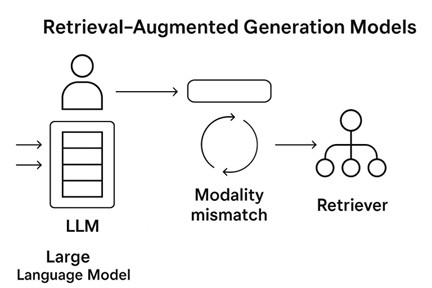
\includegraphics[width=0.72\linewidth]{volumes/pic/Picture1.2.jpg}
    \caption{Standard retrieval-augmented generation pipeline. In conventional RAG, retrieval remains externally mediated through a document index or vector store before generation. DLI proposes to move part of this retrieval logic into the model's differentiable computation path.}
    \label{fig:rag-pipeline}
\end{figure}

\section{Mathematical Framing of Differentiable Latent Indexing}
To transition from conceptual architecture to a formally analyzable model, this section expresses DLI-LLM as a minimal extension of standard Transformer notation. Let $h_t^{(\ell)} \in \mathbb{R}^{d}$ denote the hidden state at token position $t$ and layer $\ell$, following the general structure of attention-based Transformer computation \cite{Vaswani2017}. DLI augments this computation with a latent key--value memory and a differentiable routing mechanism.

\subsection{Latent Key--Value Memory}
For each layer $\ell$, define a latent memory bank:

\begin{equation}
M^{(\ell)} = \{(k_i^{(\ell)}, v_i^{(\ell)})\}_{i=1}^{N},
\end{equation}

where $k_i^{(\ell)} \in \mathbb{R}^{d_k}$ is a memory key and $v_i^{(\ell)} \in \mathbb{R}^{d_v}$ is the corresponding memory value. The memory bank may contain internal token-derived representations, document-derived embeddings, or a hybrid of both. This formulation extends differentiable memory systems by embedding the memory inside the layer-level computation rather than attaching it as a separate controller \cite{Graves2014,Graves2016,Santoro2016}.

\subsection{Query Projection}
A learned projection maps the current hidden state into a retrieval query:

\begin{equation}
q_t^{(\ell)} = W_q^{(\ell)} h_t^{(\ell)} + b_q^{(\ell)}.
\end{equation}

This query projection is analogous to attention-based addressing but is directed toward persistent latent memory rather than only toward positions within the active context window \cite{Bahdanau2016,Vaswani2017}.

\subsection{Similarity and Sparse Retrieval}
The model computes retrieval logits through a similarity function:

\begin{equation}
s_i^{(\ell)} = \frac{q_t^{(\ell)} \cdot k_i^{(\ell)}}{\sqrt{d_k}}
\end{equation}

A sparse top-$k$ selection operator restricts retrieval to the most relevant memory entries: 

\begin{equation}
\alpha_i^{(\ell)} = \frac{\exp(s_i^{(\ell)}/\tau)\mathbf{1}[i \in \operatorname{TopK}(s^{(\ell)}, k)]}{\sum_{j \in \operatorname{TopK}(s^{(\ell)}, k)} \exp(s_j^{(\ell)}/\tau)}
\end{equation}

where $\tau$ is a temperature parameter and $\alpha_i^{(\ell)}$ is the differentiable retrieval weight assigned to memory slot $i$. Product quantization may be used to approximate key search at scale \cite{Jgou2011,Johnson2021}.

\subsection{Retrieved Representation}
The retrieved latent representation is computed as a weighted sum of memory values:

\begin{equation}
r_t^{(\ell)} = \sum_{i=1}^{N} \alpha_i^{(\ell)} v_i^{(\ell)}.
\end{equation} 

This operation turns memory access into a differentiable aggregation step, preserving gradient flow through the retrieval distribution.

\subsection{Gated Fusion}
A learned gate controls the influence of retrieved memory on the evolving hidden state:

\begin{equation}
g_t^{(\ell)} = \sigma\left(W_g^{(\ell)}[h_t^{(\ell)} \parallel r_t^{(\ell)}] + b_g^{(\ell)}\right),
\end{equation}

where $[h_t^{(\ell)} \parallel r_t^{(\ell)}]$ denotes vector concatenation and $\sigma$ is the logistic sigmoid. The fused representation is then:

\begin{equation}
\tilde{h}_t^{(\ell)} = \operatorname{LayerNorm}\left(h_t^{(\ell)} + g_t^{(\ell)} \odot r_t^{(\ell)}\right).
\end{equation}

This gating operation connects DLI to conditional computation and mixture-style routing, while preserving a layer-local mechanism for regulating memory influence \cite{Lepikhin2020,Bulatov2022}.

\subsection{Training Objective}
A conceptual DLI training objective can be written as:

\begin{equation}
\mathcal{L}_{DLI} = \mathcal{L}_{LM} + \lambda_s \mathcal{L}_{sparse} + \lambda_m \mathcal{L}_{memory} + \lambda_g \mathcal{L}_{gate}
\end{equation}

where $\mathcal{L}_{LM}$ is the standard language modeling loss, $\mathcal{L}_{sparse}$ regularizes retrieval selectivity by penalizing the entropy of the allocation profile $\alpha$, $\mathcal{L}_{memory}$ regulates memory coherence or redundancy, and $\mathcal{L}_{gate}$ discourages uncontrolled reliance on retrieved values. The exact form of these terms is an empirical design question, but the formulation clarifies where future implementations may intervene.

\subsection{Gradient Flow and Optimization Continuity}
Because the sparse selection operator $\operatorname{TopK}(\cdot)$ introduces a non-differentiable boundary, gradient continuity through the retrieval pathway is maintained via the soft-max weighting allocation across the chosen partition. The partial derivative of the fused representation $\tilde{h}_t^{(\ell)}$ with respect to the memory keys $k_i^{(\ell)}$ propagates directly through the similarity scaling:

\begin{equation}
\frac{\partial \tilde{h}_t^{(\ell)}}{\partial k_i^{(\ell)}} = g_t^{(\ell)} \odot v_i^{(\ell)} \left( \frac{\partial \alpha_i^{(\ell)}}{\partial s_i^{(\ell)}} \right) \left( \frac{q_t^{(\ell)}}{\sqrt{d_k}} \right).
\end{equation}

This formalizes a continuous, uninterrupted backward pass from downstream language modeling errors directly into the latent memory coordinates, allowing the index structure to co-evolve with parametric transformations without a separate optimization loop.

\textbf{Figure}~\ref{fig:gradient-pathways} illustrates how gradients propagate through the attention and retrieval pathways during training.

\begin{figure}
    \centering
    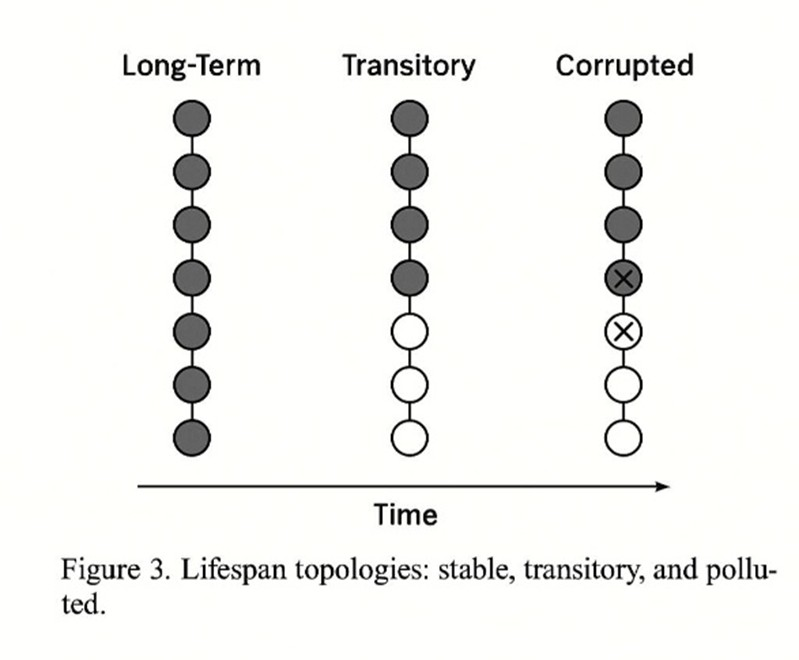
\includegraphics[width=0.72\linewidth]{volumes//pic/Picture1.3.jpg}
    \caption{Gradient pathways in Differentiable Latent Indexing. Query projection, similarity computation, sparse retrieval weighting, routed memory integration, and gated fusion remain within the differentiable computation graph, allowing latent memory to co-evolve with Transformer parameters.}
    \label{fig:gradient-pathways}
\end{figure}

\section{Algorithmic Specification and Implementation Blueprint}
To operationalize the retrieval mechanism described above, Algorithm~\ref{alg:dli-loop} specifies a single DLI retrieval step within one Transformer layer.

\begin{center}
\fbox{%
\begin{minipage}{0.92\linewidth}
\textbf{Algorithm 1}: Differentiable Latent Indexing Loop\label{alg:dli-loop}

\textbf{Input:} hidden state $h_t^{(\ell)}$, latent memory $M^{(\ell)} = \{(k_i^{(\ell)}, v_i^{(\ell)})\}_{i=1}^{N}$, parameters $W_q^{(\ell)}$, $W_g^{(\ell)}$, top-$k$ value, temperature $\tau$.

\textbf{Output:} fused representation $\tilde{h}_t^{(\ell)}$.

\begin{enumerate}
    \item Compute retrieval query: $q_t^{(\ell)} \leftarrow W_q^{(\ell)}h_t^{(\ell)} + b_q^{(\ell)}$.
    \item Compute similarity scores: $s_i^{(\ell)} \leftarrow q_t^{(\ell)} \cdot k_i^{(\ell)} / \sqrt{d_k}$.
    \item Select top-$k$ memory slots according to $s_i^{(\ell)}$.
    \item Compute retrieval weights: $\alpha^{(\ell)} \leftarrow \operatorname{softmax}(s^{(\ell)}/\tau)$ over selected slots.
    \item Retrieve latent value: $r_t^{(\ell)} \leftarrow \sum_i \alpha_i^{(\ell)}v_i^{(\ell)}$.
    \item Compute routing gate: $g_t^{(\ell)} \leftarrow \sigma(W_g^{(\ell)}[h_t^{(\ell)} \parallel r_t^{(\ell)}] + b_g^{(\ell)})$.
    \item Fuse retrieved memory with hidden state: $\tilde{h}_t^{(\ell)} \leftarrow \operatorname{LayerNorm}(h_t^{(\ell)} + g_t^{(\ell)} \odot r_t^{(\ell)})$.
    \item Return $\tilde{h}_t^{(\ell)}$.
\end{enumerate}
\end{minipage}}
\end{center}

Although this paper is theoretical, an implementable DLI prototype would require four design stages.

\subsection{Memory Construction}
Document embeddings, token representations, or intermediate hidden states would be transformed into latent key--value banks. Product quantization could then be applied to compress memory and enable approximate retrieval at scale \cite{Jgou2011,Johnson2021}.

\subsection{Quantized Latent Indexing Mechanics}
To prevent the $\operatorname{TopK}$ operations from scaling linearly $\mathcal{O}(N)$ with the size of the latent memory repository, the key space is structured using Product Quantization (PQ). The high-dimensional key space $\mathbb{R}^{d_k}$ is decomposed into $M$ orthogonal subspaces:

\begin{equation}
\mathbb{R}^{d_k} = \mathbb{R}^{d_s} \times \mathbb{R}^{d_s} \times \dots \times \mathbb{R}^{d_s},
\end{equation}

where $d_s = d_k / M$. Each subspace is quantized into $K^*$ centroids using a learned codebook. During the forward pass, the query projection $q_t^{(\ell)}$ is similarly sliced into $M$ sub-vectors. Similarity estimation $s_i^{(\ell)}$ is then executed via asymmetric distance computation (ADC) using pre-calculated look-up tables. This reduces the computational overhead of the internalized retrieval phase to a collection of parallel cache lookups, maintaining a highly bounded inference budget.

\subsection{Layer Integration}
A DLI block would be inserted after self-attention or between attention and feed-forward sublayers. The routing gate would determine whether retrieved values should influence the hidden state. This placement allows DLI to function as a memory-aware extension of Transformer computation rather than as a separate retrieval pipeline.

\subsection{Training and Fine-Tuning}
Training would jointly optimize language modeling, retrieval selectivity, memory coherence, and gating behavior. In a pre-training setting, memory slots could evolve with the model. In a fine-tuning setting, selected memory banks could be frozen, swapped, or domain-adapted.

\subsection{Inference Behavior}
During inference, DLI could operate through frozen or partially updateable memory. Sparse top-$k$ retrieval would limit computational overhead. Memory swapping could support domain-specific deployment, while gating thresholds could regulate when latent memory is allowed to influence generation.

\subsection{Evaluation Plan}
A future empirical study should compare DLI-augmented models against baseline Transformers, RAG models, kNN-LM variants, and memorizing transformers. Evaluation should include latency overhead, retrieval precision, hallucination rates, long-context coherence, memory saturation, and ablation studies that disable routing, memory access, or quantization independently.

\section{Comparative Literature Analysis}
\textbf{Table}~\ref{tab:comparative-architectures} summarizes the position of DLI relative to adjacent architectures.

\begin{table}
\centering
\small
\begin{tabular}{p{0.26\linewidth}p{0.34\linewidth}p{0.30\linewidth}}
\hline
\textbf{Architecture} & \textbf{Relation to DLI} & \textbf{Limitation Relative to DLI} \\
\hline
Retrieval-Augmented Generation & Combines parametric generation with non-parametric retrieval \cite{Lewis2021}. & Retrieval is typically external to the Transformer computation graph. \\
$k$NN-LM & Interpolates language-model predictions with nearest-neighbor lookup \cite{Khandelwal2020}. & Retrieval is post-hoc and not trained as an internal layer function. \\
Memorizing Transformers & Store and retrieve recent key--value representations \cite{Wu2022}. & Memory improves context use but remains distinct from document-level latent unification. \\
Neural Turing Machines / DNC & Demonstrate differentiable memory addressing \cite{Graves2014,Graves2016}. & Designed as general memory controllers rather than layer-native LLM retrieval modules. \\
Memory-Augmented Neural Networks & Support rapid assimilation of new examples \cite{Santoro2016}. & Primarily oriented toward few-shot learning rather than Transformer-internal retrieval. \\
Recurrent Memory Transformer & Uses memory tokens for long-sequence processing \cite{Bulatov2022}. & Memory persistence is present, but explicit latent key--value retrieval control is limited. \\
Dense Passage Retrieval / RocketQA & Optimizes learned representations for retrieval \cite{Qu2021}. & Retrieval occurs outside the model's internal forward computation. \\
Product-Quantized Vector Search & Provides scalable approximate search \cite{Jgou2011,Johnson2021}. & Supplies retrieval infrastructure but not a cognitive or Transformer-layer architecture. \\
\hline
\end{tabular}
\caption{Comparative analysis of memory-augmented and retrieval-integrated architectures.}
\label{tab:comparative-architectures}
\end{table}

\section{Discussion}
The DLI-LLM architecture reframes how memory is conceptualized in Transformer-based systems. By integrating retrieval into the forward pass, the model collapses the traditional separation between reasoning and recall. This aligns with cognitive architecture research that treats memory, control, learning, and representation as interdependent properties of intelligent systems \cite{Sun2004}.

\subsection{Cognitive Implications}
Embedding differentiable latent memory directly within Transformer layers positions retrieval as a native cognitive operation rather than an external API call. This shift parallels earlier insights from memory-augmented neural networks and differentiable memory systems \cite{Graves2014,Graves2016,Santoro2016}, but extends them by proposing a unified latent space where token-derived representations and document-derived vectors can coexist. The resulting architecture moves toward cognitive completeness by enabling context-dependent recall, internal evidence arbitration, and persistent cross-layer memory flow.

\subsection{Learning Dynamics and Adaptation}
DLI-LLM suggests new possibilities for lifelong and continual learning. If memory slots can be updated incrementally, the model may integrate new documents without full retraining, a capability related to recurrent memory systems and neural semantic encoders \cite{Bulatov2022,Munkhdalai2017}. However, this advantage introduces challenges. Latent memory may overfit internal distributions, memory slots may saturate, and retrieval may become redundant without pruning, quantization, or regularization \cite{Jgou2011,Johnson2021}.

\subsection{Bias, Safety, and Privacy Considerations}
The integration of retrieval into model computation raises safety concerns. Frozen memory layers may preserve sensitive information, creating privacy risks. Internal retrieval may reinforce biased representations. Latent memories, once implicitly learned, may be harder to inspect than externally retrieved documents. These risks parallel issues in retrieval-augmented systems but are amplified by the opacity of internalized memory \cite{Lewis2021}.

\subsection{Architectural Control and Gating Mechanisms}
A central feature of DLI-LLM is the routing gate. The gate mediates the integration of retrieved values into the hidden state, determines how retrieval influences inference, and regulates cross-layer propagation. Conceptually, this places gating at the core of cognitive control: the architecture must learn not only what to retrieve, but also when retrieval should matter. \textbf{Figure}~\ref{fig:gating-control} illustrates this control path.

\begin{figure}
    \centering
    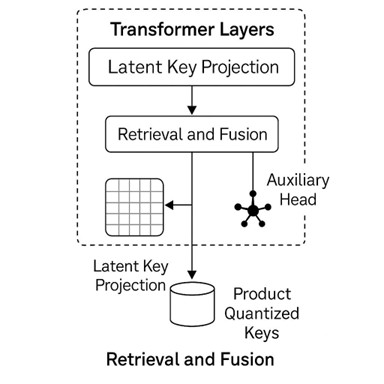
\includegraphics[width=0.72\linewidth]{volumes/pic/Picture1.4.jpg}
    \caption{Training flow and gating control in DLI-LLM. Product-quantized key--value lookup, attention fusion, routing gates, and gradient-based memory adaptation interact across Transformer blocks.}
    \label{fig:gating-control}
\end{figure}

\subsection{Toward Cognitive-Complete Transformer Architectures}
DLI-LLM argues for reconsidering memory-augmented Transformers not as storage-bound enhancements, but as components of a broader approach to machine cognition. In this view, retrieval is not merely a way to extend context length; it is a candidate mechanism for internal evidence selection, representational persistence, and adaptive control. This aligns with the broader desideratum that cognitive architectures should integrate memory, learning, representation, and control into a coherent system \cite{Sun2004}.

\section{Conclusion}
Differentiable Latent Indexing proposes that retrieval can be moved from the periphery of language-model architecture into the differentiable interior of Transformer computation. The framework introduced here formalizes this idea through latent key--value memory, query projection, sparse retrieval, gated fusion, and a conceptual training objective. It also defines falsifiable propositions, expected benefits, and plausible failure modes.

The paper does not claim that DLI-LLM has already been implemented or empirically validated. Its contribution is theoretical: it clarifies what such an architecture would require, how it differs from existing retrieval and memory-augmented models, and what future experiments would need to test. As the first volume in the \textit{Latent Cognition Trilogy}, this article establishes memory as the initial boundary condition for a broader investigation into artificial cognition.

\bibliographystyle{plain}
\bibliography{references.bib}